\chapter{Разработка принципов создания инструмента проектирования архитектуры}\label{ch:ch4}
Проектирование архитектуры автоматизированной системы является наиболее абстрактным и наиболее идеализированным представлением системы, которое должно обеспечивать выполнение следующих свойств:
\begin{enumerate}
\item элементы архитектуры должны быть слабо связаны таким образом, чтобы разложив на декомпозицию элементов, поток информации, проходящий по контурам был минимальным и не замыкался;
\item должно соблюдаться свойство тестируемости, т.е. при проверки работы функций системы должен быть установлен факт правильной работы;
\item должна соблюдаться возможность идентификации неисправных частей системы путем диагностики;
\item должно соблюдаться свойства восстановления системы в кратчайшие сроки с экономически обоснованной стоимостью ремонта;
\item должно соблюдаться свойство надежности;
\item система должна быть проста в обслуживании и проста в эксплуатации, не требовать высокой квалификации и повышения квалификации обслуживающего персонала;
\item система и ее составляющие элементы должны быть безопасны в эксплуатации, должны соблюдать требования охраны труда и техники безопасности;
\item система должны быть обеспечена защитой от вандализма и неавторизованных пользователей;
\item система должна проектироваться с учетом эффективности в отношении затрачиваемых ресурсов в  операционном процессе;
\item система должна уметь выстаиваивать новые конфигурации, создавать новые настройки для работы с другими технологическими процессами;
\item система должна уметь функционально расширяться, т.е. в логика работы должна уметь дополняться дополнительными функциональными возможностями системы;
\item система должны быть готова к устойчивому масштабированию системы, таким образом, чтобы увеличение размера объекта автоматизации не требовало высоких затрат и не сводила к неустойчивому состоянию базовую модель системы;
\item система должна быть открытой, таким образом, чтобы можно было заменить один модуль системы на аналогичный модуль другого производителя, а интеграция модулей происходила без чрезмерных конфликтов и проблем;
\item система должна стремиться к максимально продолжительному жизненному циклу без значительного устаревания, который должен обновлять аппаратные и программные компоненты;
\item система должна устанавливаться и вводиться в эксплуатацию за минимальное время.
\end{enumerate}

Таким образом, модель должна соблюдать перечисленные выше технические требования.

\section{Общие положения}\label{sec:ch3/sect1}

Цель - разработать алгоритм в соответствии с вышеописанными принципами:
для этого необходимо входным переменным $X = {x_1, x_2, ..., x_n}$ поставить в соответствие выходные $Y = {y_1, y_2, ..., y_n}$. Первым неоьходимоым принципом является преобразование базы знаний. Данная операция изображена на Рисунке ~\cref{fig:NNprin}.
\begin{figure}[ht]
    \centerfloat{
        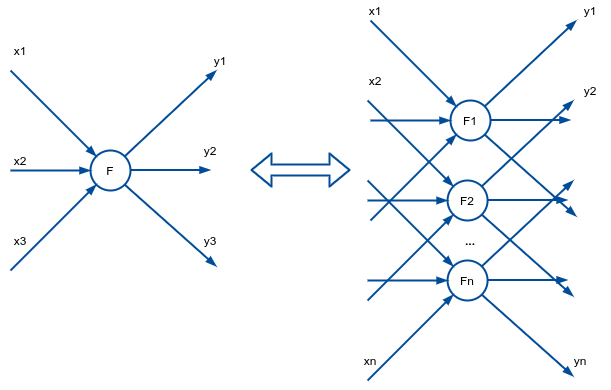
\includegraphics[scale=0.8]{Dissertation/images/DISSER-18.png}
    }
    \caption{Структура принципа преобразования}\label{fig:NNprin}
\end{figure}

Принцип реализации сводится к адаптации информации, сформированной на базе фактов с пользовательским запросом на обработку и выдачу рекомендаций по проектированию. Общая схема движения информационного потока представлена на Рисунке~\cref{fig:Dataflow} 

\begin{figure}[ht]
    \centerfloat{
        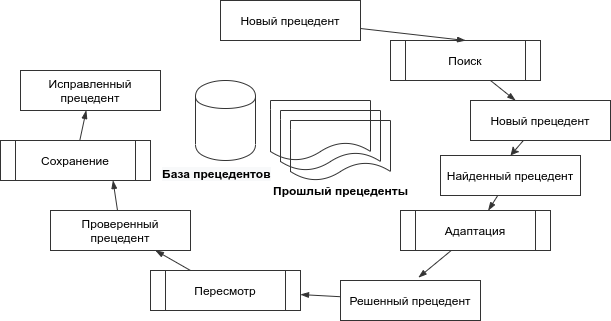
\includegraphics[scale=0.8]{Dissertation/images/DISSER-16.png}
    }
    \caption{Структура принципа преобразования}\label{fig:Dataflow}
\end{figure}






\section{Разработка принципов создания специального математического и алгоритмического обеспечения проектирования архитектуры  }\label{sec:ch3/sect2}

Основным принципом создания системы поддержки принятия решений назовем модуль функциональной работы нейронной сети на основе нечеткой логики.
Нейронная сеть с нечеткой логикой должна аппроксимировать некоторый функционал в соответствии со следующими принципами:
\begin{enumerate}
	\item множество входных параметров переменных $X = {x_1, x_2, ..., x_n}$, характеризующие объект получения рекомендации,
	\item множество выходных переменных $Y = {y_1, y_2, ..., y_n}$, характеризуюших рекомендацию по объекту проектирования,
	\item множество лингвистических переменных термов $A = {a_j, a_{j+1}, a_m}$, которые являются мерой соотнесения с нечеткой функцией классификации переменных $x_i$,
	\item множество лингвистических переменных термов $B = {b_j, b_{j+1}, b_m}$, которые являются мерой соотнесения с нечеткой функцией классификации переменных $y_i$,
	\item функция принадлежности ~\cref{eq:equation45},
	\item матрица знаний, согласно Рисунку ~\cref{fig:KBase}.
\end{enumerate}


После принципа преобразования получаем следующую систему однородных нелинейных преобразований
\begin{equation}
    \label{eq:equation57}
     \left\{\begin{array}{ll} 
    y_1 = F_1(X,W,C,\Psi) \textrm{,} 
    \\ y_2 = F_2(X,W,C,\Psi)  \textrm{,}
    \\ ... 
     \\ y_n = F_n(X,W,C,\Psi) 
      & \end{array} \right. \]
\end{equation}

где $X = {x_1, x_2, ..., x_n}$ - вектор входный переменных, описывающих систему,

$W$ - вектор весовых коэффициентов продукционных правил,

$C,\Psi$ - вектор функций принадлежностей лингвистических термов.


Обучающая выборка задается в виде пары $(X^p, Y^p)$, принцип поиска эвристического процесса обучения может быть описани следущим образом
\begin{equation}
    \label{eq:equation58}
    \begin{alignedat}{2}
        \sum_{p=1}^L[F_1(X^p,W,C,\Psi) - y_1^p]^2 + \\
        + \sum_{p=1}^L[F_1(X^p,W,C,\Psi) - y_2^p]^2 +  ... \\
       ... +  \sum_{p=1}^L[F_1(X^p,W,C,\Psi) - y_p^p]^2 = \\
        = \sum_{j = 1}^q{\sum_{p=1}^L{[F_j(X^p,W,C,\psi) - y^p_j]^2}}
        = min\{W,C,\Psi\}
    \end{alignedat}
\end{equation}

Принцип создания обучающей выборки состоит в том, чтобы предъявить факты и уже известный продукционный вывод для обучения, чтобы нейронная сеть могла начать процесс апроксимации функционала соответствия, опираясь на эвристический поиск соответствия.
Принцип работы функциональной схемы обработки и формирования эвристического соответствия входному и выходному вектору переменных приведен на Рисунке ~\cref{fig:FL}
\begin{figure}[ht]
    \centerfloat{
        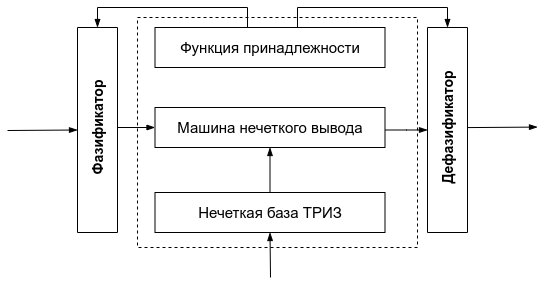
\includegraphics[scale=0.8]{Dissertation/images/DISSER-9.png}
    }
    \caption{Структура принципа преобразования}\label{fig:FL}
\end{figure}

Таким образом основным принципом формирования модели поддержки принятия решений является эвристический аппроксиматор функционала продукционного вывода, функционала эвристического соответствия между входным вектором и выходным.

\subsection{Выбор основного принципа реализации модели}\label{subsec:ch3/sect2/sub1}

На Рисунке~\cref{fig:FLbase} представлен основной принцип реализации модели эвристического соответствия между входными переменными и выходными.
\begin{figure}[ht]
    \centerfloat{
        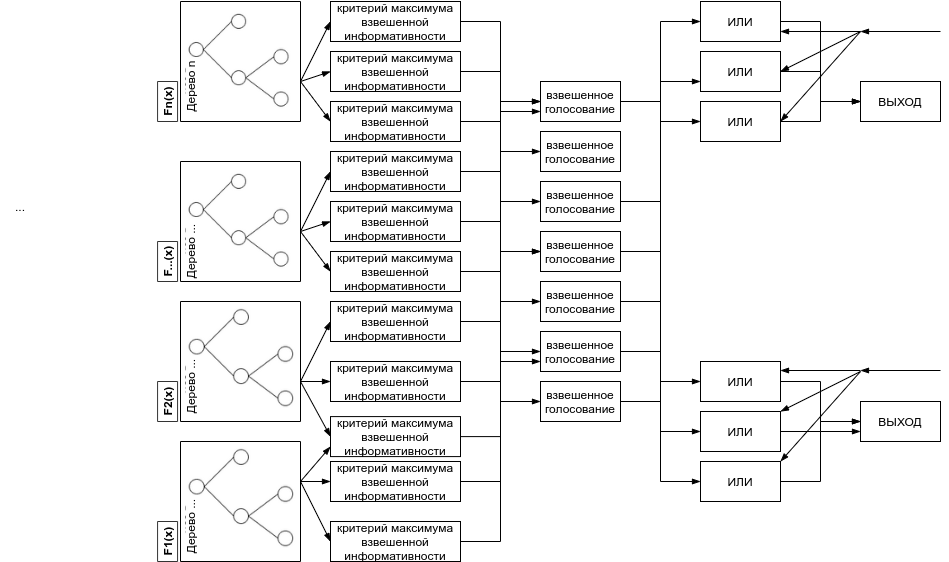
\includegraphics[scale=0.8]{Dissertation/images/DISSER-10.png}
    }
    \caption{Структура принципа формирования эвристического соответствия}\label{fig:FLbase}
\end{figure}

Структура основного принципа реализации модели состоит из следующих этапов:
\begin{enumerate}
	\item формирование данных для обучения,
	\item настройка нечетких функционалов принадлежности,
	\item обучение по соревнованию,
	\item удаление продукционных правил, не прошедшие критерий соответствия,
	\item комбинирование правил согласно теории множеств,
	\item финальная настройка соответствия нечетких функционалов и входных и выходных параметров на основе ошибки. 
\end{enumerate}

Настройка функционала принадлежности
\begin{equation}
    \label{eq:equation59}
     y_i^{k}(x) = e^{\frac{-(x_i-x_i)}{2\sigma_i^2}}
\end{equation}

Обучение по соревнованию может быть представлено в виде
\begin{equation}
    \label{eq:equation60}
     \bigtriangleup c_\omega(t) = \eta(t)(x-c_\omega(t))
\end{equation}

где $\eta(t)$ - градиент обучения.

Шаг градиента выбирается произвольным образом, эвристически, затем исправляется в соответствии с откликом в виде ошибки обучения. Соревновательный алгоритм оценивает две матрицы весовых характеристик параметров важности фактов, а также качество связей между матрицами. В этом месте допускается использование и полноценного алгоритма нейронной сети, таких, как, например, генеративно-состязательные нейронные сети~\cite{Goodfellow}.
\begin{equation}
    \label{eq:equation61}
     \bigtriangleup \omega = y_j(y_j - \omega_{ji})
\end{equation}

Комбинирование правил выполняется с помощью экспертных знаний. Окончательный этап формирования принципа формирования соответствия строится на основании функции поправки ошибок
\begin{equation}
    \label{eq:equation62}
     e_t = (y_t - d_k)
\end{equation}

Таким образом, основным принципом формирования эвристического функционала принадлежности являются этапы формирования знаний и поправки градиента обучения с помощью возмущаеющего сигнала ошибки, это формирует функционал соответствия в виде нелинейной адаптивной комбинированной системы с возмущением. 
На Рисунке ~\cref{fig:FLmetrics} представлен основные принципы расчета расстояний. 
\begin{figure}[ht]
    \centerfloat{
        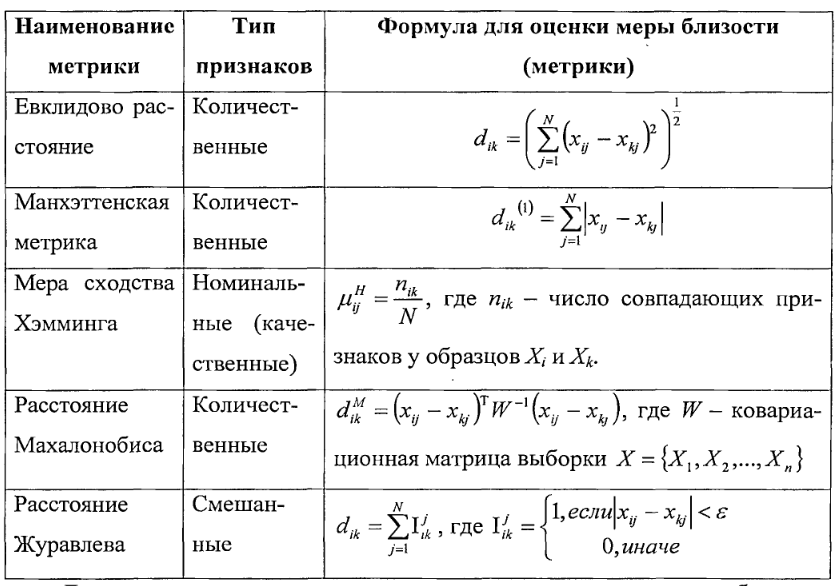
\includegraphics[scale=0.65]{Dissertation/images/DISSER-11.png}
    }
    \caption{Структура принципа расчета расстояния}\label{fig:FLmetrics}
\end{figure}
\subsection{Назначение специального математического и алгоритмического обеспечения}\label{subsec:ch3/sect2/sub1}
Назначение системы состоит в поддержки принятия решений на этапе проектирования архитектура программного обеспечения.

\section{Функциональные возможности программного обеспечения}\label{sec:ch3/sect3}

Функциональные возможности проганммного обеспечения на текущем этапе работ позволяет вводит в пользовательском режиме информацию о характеристиках планируемой архитектуры программного обеспечения и выводит рекомендованную структуру организации и необходимую инфраструктуру для проектирования. Система впоследствии может быть дополнена модулями анализа кода, а также модулями анализа отношений между сущностями и таблицами в базе данных.

\subsection{Ввод данных}\label{subsec:ch3/sect3/sub1}
Ввод данных происходит по заполнению специальной формы представленной на Рисунках~\cref{fig:ui-1,fig:ui-2,fig:ui-3,fig:ui-4,fig:ui-5,fig:ui-6}. 
\begin{figure}[ht]
    \centerfloat{
        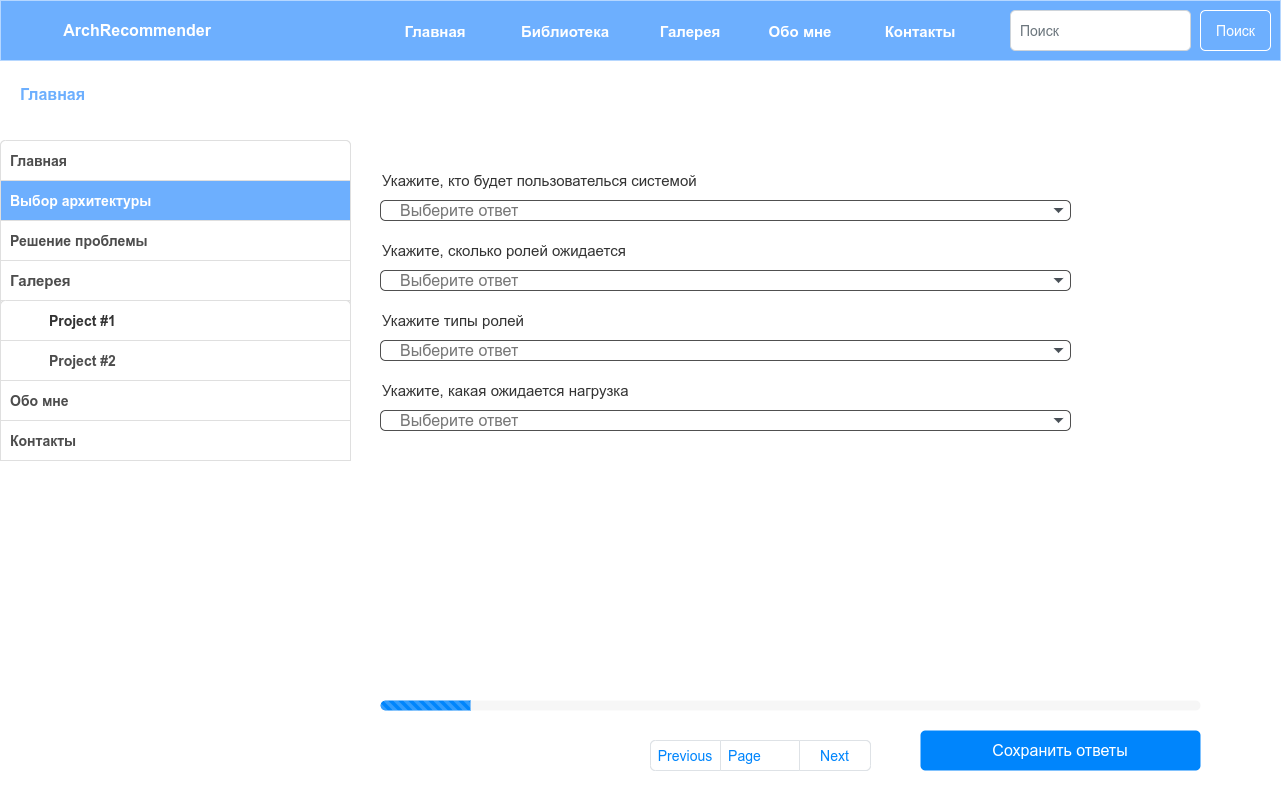
\includegraphics[scale=0.40]{Dissertation/images/DISSER-21.png}
    }
    \caption{Пользовательский ввод данных}\label{fig:ui-1}
\end{figure}

\begin{figure}[ht]
    \centerfloat{
        
\includegraphics[scale=0.40]{Dissertation/images/DISSER-22.png}
    }
    \caption{Пользовательский ввод данных}\label{fig:ui-2}
\end{figure}

\begin{figure}[ht]
    \centerfloat{
        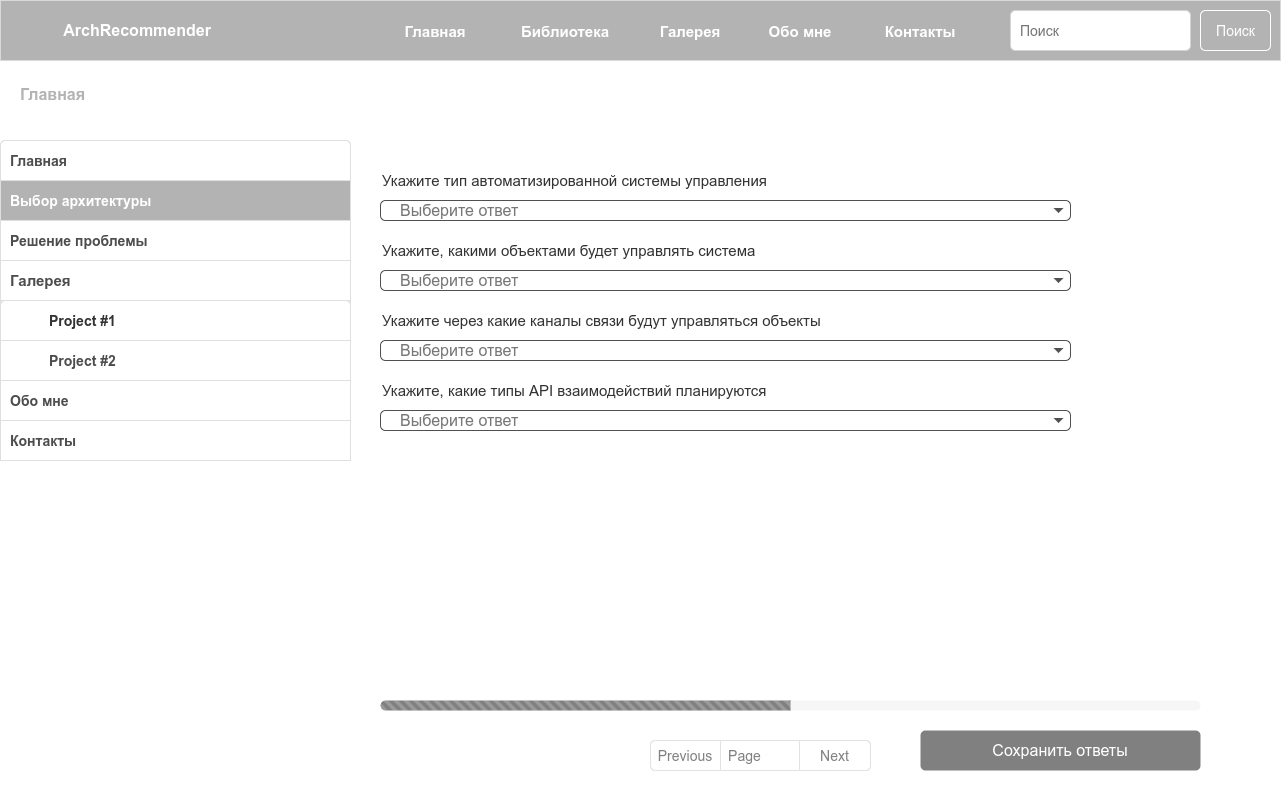
\includegraphics[scale=0.40]{Dissertation/images/DISSER-23.png}
    }
    \caption{Пользовательский ввод данных}\label{fig:ui-3}
\end{figure}

\begin{figure}[ht]
    \centerfloat{
        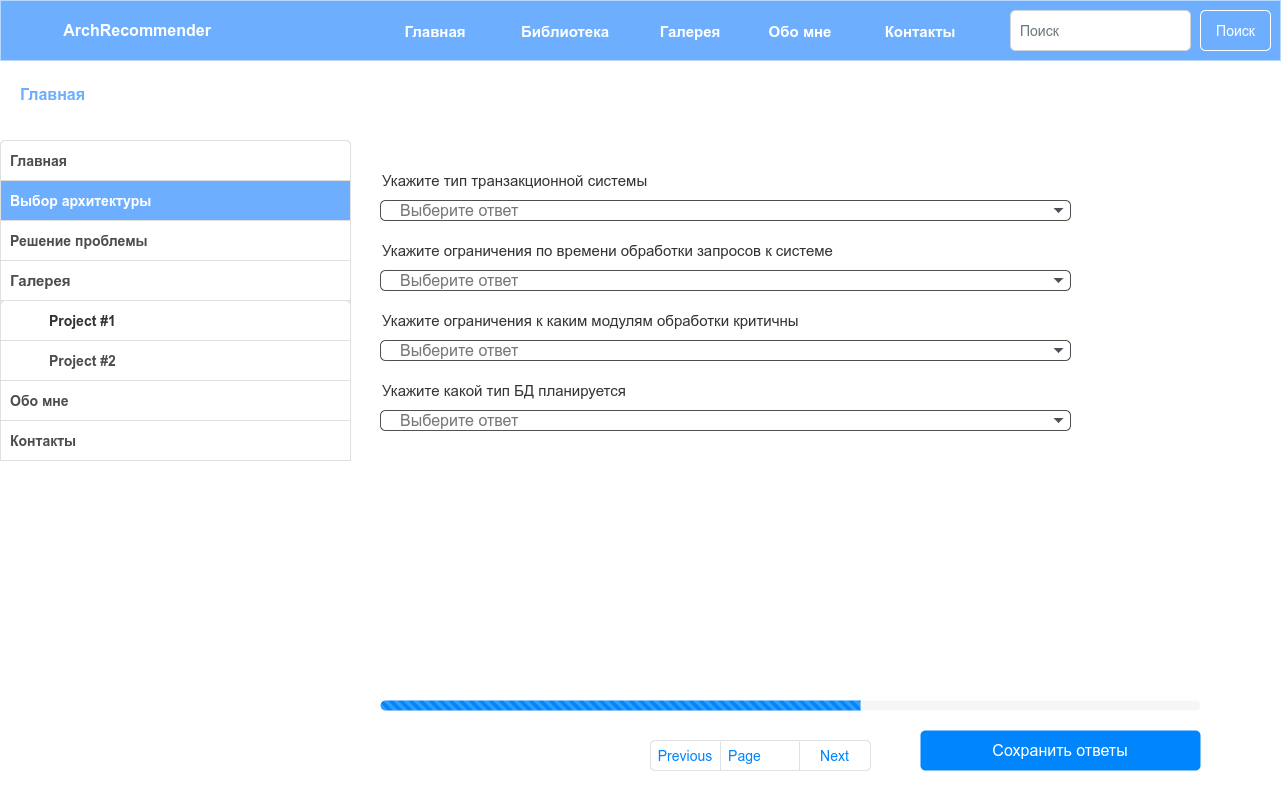
\includegraphics[scale=0.40]{Dissertation/images/DISSER-24.png}
    }
    \caption{Пользовательский ввод данных}\label{fig:ui-4}
\end{figure}

\begin{figure}[ht]
    \centerfloat{
        
\includegraphics[scale=0.40]{Dissertation/images/DISSER-25.png}
    }
    \caption{Пользовательский ввод данных}\label{fig:ui-5}
\end{figure}

\begin{figure}[ht]
    \centerfloat{
        
\includegraphics[scale=0.40]{Dissertation/images/DISSER-26.png}
    }
    \caption{Пользовательский ввод данных}\label{fig:ui-6}
\end{figure}


Перечень параметров указан в Таблице \cref{tab:tab_pref} приложения~\cref{app:A2}.

\subsection{Обработка данных}\label{subsec:ch3/sect3/sub2}

На Рисунке ~\cref{fig:FLprocess} представлен процесс обработки данных нейронной сетью на основе нечеткого вывода. 
\begin{figure}[ht]
    \centerfloat{
        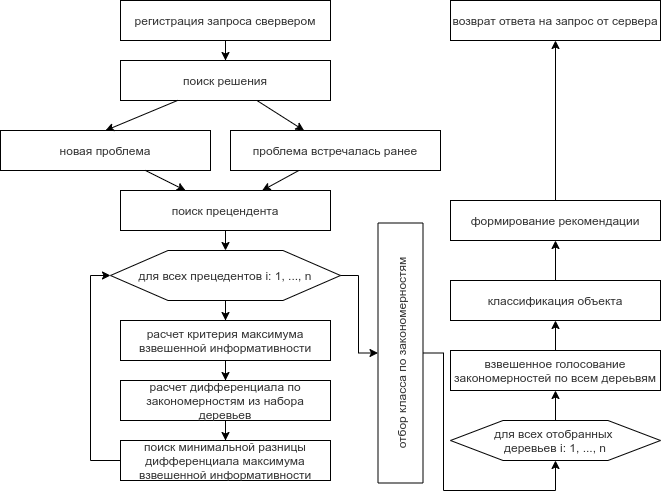
\includegraphics[scale=0.6]{Dissertation/images/DISSER-12.png}
    }
    \caption{Структура обработки информации}\label{fig:FLprocess}
\end{figure}
На Рисунке ~\cref{fig:NNprocess1} представлен процесс обработки данных нейронной сетью на основе нечеткого вывода. 
\begin{figure}[ht]
    \centerfloat{
        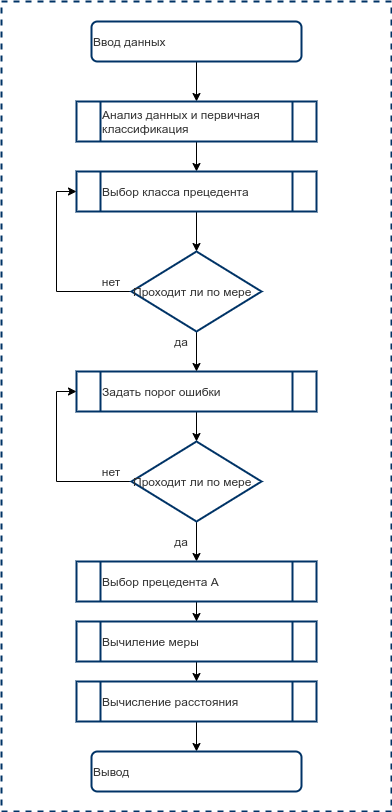
\includegraphics[scale=0.8]{Dissertation/images/DISSER-28.png}
    }
    \caption{Структура обработки информации}\label{fig:NNprocess1}
\end{figure}
На Рисунке ~\cref{fig:NNprocess2} представлен процесс обработки данных нейронной сетью на основе нечеткого вывода. 
\begin{figure}[ht]
    \centerfloat{
        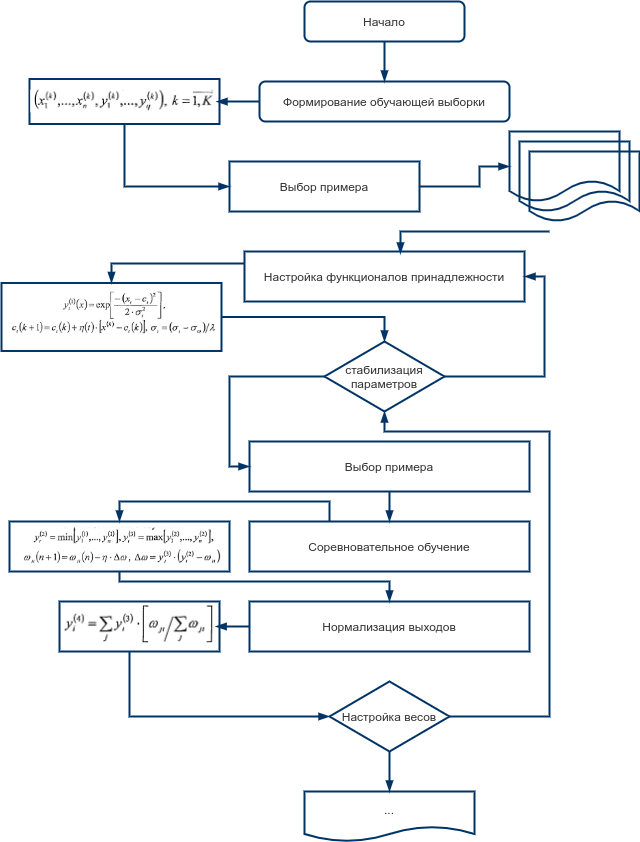
\includegraphics[scale=0.8]{Dissertation/images/DISSER-29.png}
    }
    \caption{Структура обработки информации}\label{fig:NNprocess2}
\end{figure}
На Рисунке ~\cref{fig:NNprocess3} представлен процесс обработки данных нейронной сетью на основе нечеткого вывода. 
\begin{figure}[ht]
    \centerfloat{
        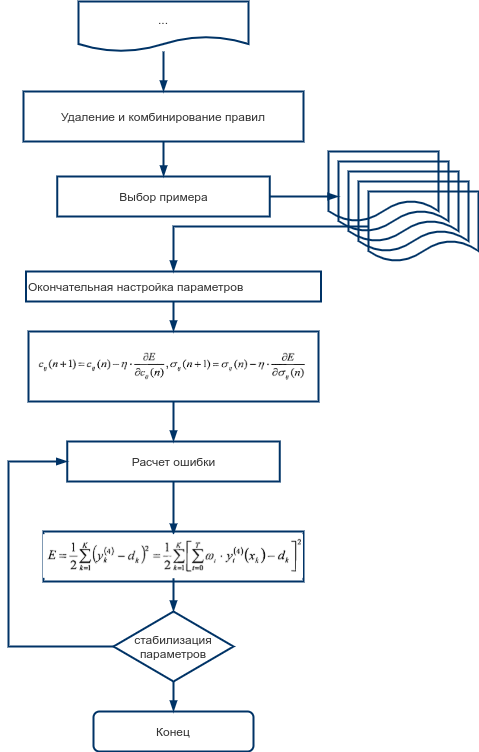
\includegraphics[scale=0.8]{Dissertation/images/DISSER-30.png}
    }
    \caption{Структура обработки информации}\label{fig:NNprocess3}
\end{figure}

\subsection{Отчеты и анализ данных}\label{subsec:ch3/sect2/sub3}
Результат работы программы представлен на Рисунке~\cref{fig:res}.
\begin{figure}[ht]
    \centerfloat{
        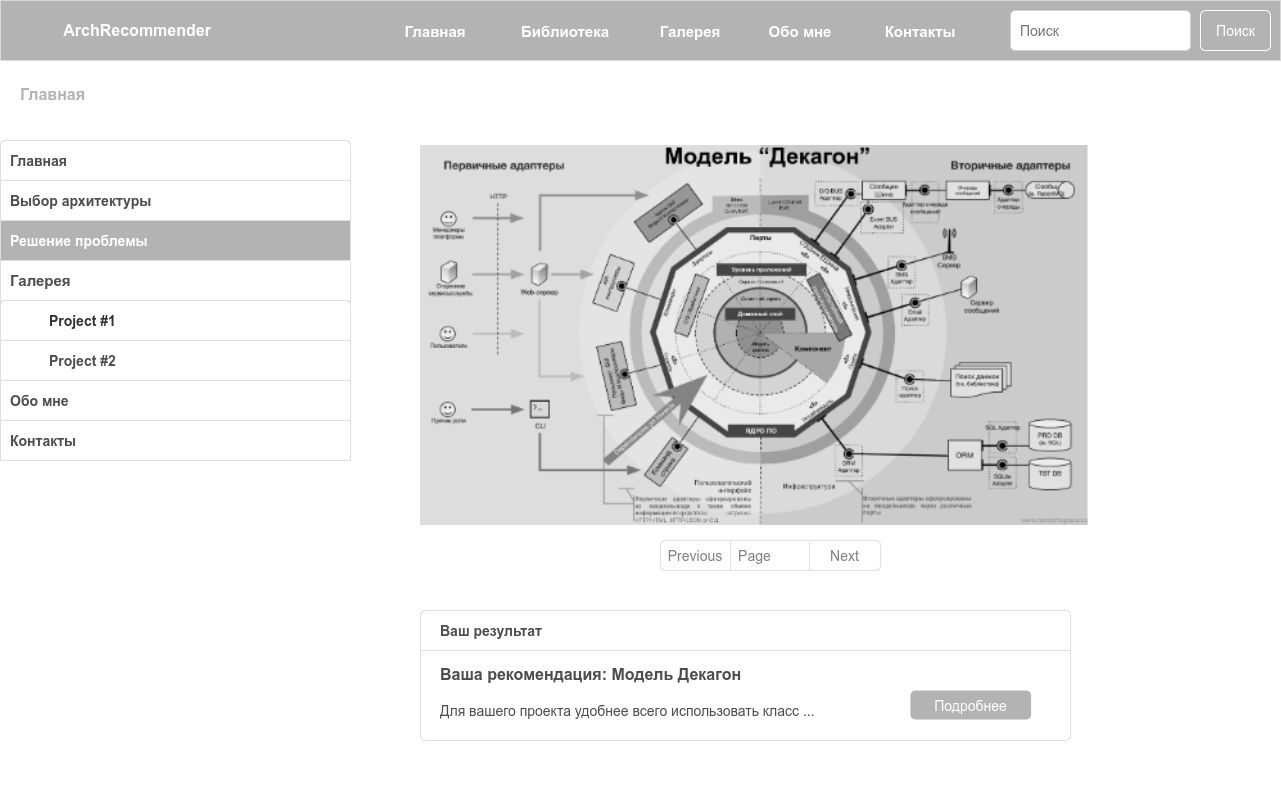
\includegraphics[scale=0.4]{Dissertation/images/DISSER-27.png}
    }
    \caption{Структура вывода информации}\label{fig:res}
\end{figure}
На Рисунке ~\cref{fig:res1} представлен результат обработки данных нейронной сетью на основе нечеткого вывода. 
\begin{figure}[ht]
    \centerfloat{
        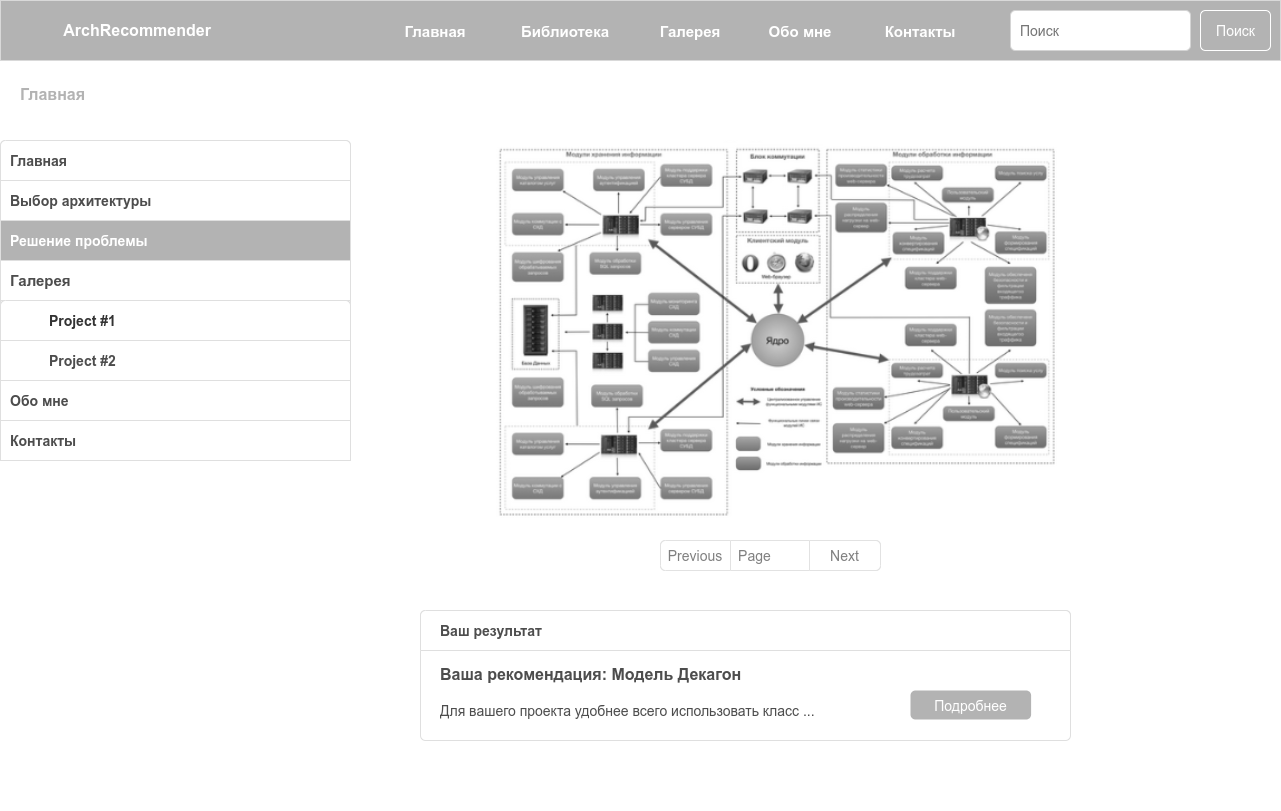
\includegraphics[scale=0.4]{Dissertation/images/DISSER-31.png}
    }
    \caption{Структура вывода информации}\label{fig:res1}
\end{figure}
\subsection{Алгоритм оценки надежности разработанного специального математического и алгоритмического обеспечения}\label{sec:ch3/sect3/sub3}

Разработанная модель специального математического и алгоритмического обеспечения для задач автоматизации процесса поддержки принятий решений относительно разработки архитектуры программного обеспечения отвечает параметрам надежности согласно следующим критериям оценки:
\begin{enumerate}
    \item энтропийный критерий,
    \item статистический критерий отказа,
    \item групповой критерий надежности.
\end{enumerate}

Рассмотрим энтропийный критерий надежности относительно модели поддержки принятий решений. Объект представляется, как система поддержки принятий решений, которая взаимодействует с окружающими ее объектами и физическим миром. Данное взаимодействие может быть представлено с помощью веществ и энергий, которые в процессе взаимодействия с объектом вызывают изменеия состояний. При таких изменениях происходят изменения состояний параметров и переменных работы самого объекта, в процесс взаимодействия объекта со средой воздействия. Такие изменения влияют на равновесие, стционарность обработкиинформации, стационарность работы объекта, необратимость процессов, работоспособность, могут приводить к возникновению отказов. Рассмотрим процесс изменений состояний информации в системе с точки зрения информационной энтропии процессов.
Пусть выражение
\begin{equation}
    \label{eq:equation61}
     H = -\sum_{i=1}^n{P_ilogP_i}
\end{equation}

описывает величину неопределенности в информационном потоке сообщений.

Пусть, выражение
\begin{equation}
    \label{eq:equation62}
     \int \mathrm{\frac{\partial S}{\partial t}}\,\mathrm{d}\tau
\end{equation}

описывает принцип возрастания энтропии в потоке и будет преобразовано к виду и описывает изменение энтропии в системе.
\begin{equation}
    \label{eq:equation63}
     -\frac{\partial(\rho S)}{\partial t} + \biguptriangle (\rho S v) = \theta
\end{equation}

Рассмотри задачу оценки надежности с точки зрения задачи оценки максимума производства энтропии, где основным принципом является феномен диссипации энергии в термодинамических системах. Изменения состояния в системе представим в иде классической модели марковских процессов и уравнений Колмогорова. Данная система дифференциальных уравнений представляет изменения состояния объекта, как некоторый неоднородный марковский процесс чистого размножения с дискретным числом состояний и непрерывным временем
\begin{equation}
    \label{eq:equation64}
     \left\{\begin{array}{ll} 
    \frac{dP_1(t)}{dt} = - \lambda(t)_1 P_1(t) 
    \\ \frac{dP_i(t)}{dt} = - \lambda(t)_{i-1} P_{i-1}(t) - \lambda(t)_i P_i(t)
    \\...
    \\ \frac{dP_n(t)}{dt} = -\lambda(t)_{n-1} P_{n-1}(t)
     \forall{t} \geq t_0
      & \end{array} \right. \]
\end{equation}

где  P_1(0) = 1, P_i(0) = 0, i \in \{2,3,...,n\}.

Уравнение энтропии  для такой системы примет следующий вид
\begin{equation}
    \label{eq:equation62}
     H(t)_k = - \int_0^t \mathrm{P_k(t)log(P_k(t))}\,\mathrm{d}t
\end{equation}

где $P_k(t)$ - вероятность отказа в $k$-м состоянии в момент времени $t$.




Рассмотрим задачу анализа надежности системы с точки зрения моделирования группового отказа в системе. 

\section{Выводы по главе}\label{sec:ch3/conc}
В результате проведенной работы в данной главе были решены следующие задачи:
\begin{enumerate}
    \item проанализированы проблемы процесса обработки информации, 
    \item продемонстрирован механизм сбора информации, проведена организация сбора информации от пользователя о системе, планируемой к проектированию,
    \item определены структура, состав и характеристика входных наборов переменных, для которых составляется рекомендация,
    \item продемонстрирована алгоритмическая реализация процесса сбора, обработки информации, процесса параметризации внутреннего механизма создания рекомендаций,
    \item продемонстрирована алгоритмическая структура реализации работы нейронной сети на основе нечеткого вывода.
\end{enumerate}

В данной главе предоставлено описание пользовательского интерфейса и структуры ввода и вывода информации. Систему поддержки принятия решений следует дополнить функционалом более детального анализа по качеству отношений между сущностями. Также следует разработать механизм классификации иерархии классов в проекте.

\clearpage
